\documentclass{article}
\usepackage{amsmath,amssymb,graphicx, tikz}

\begin{document}

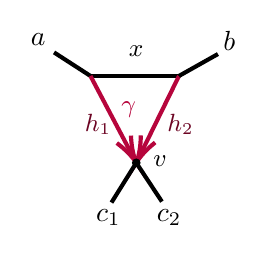
\begin{tikzpicture}[x=0.75pt,y=0.75pt,yscale=-0.9,xscale=0.9]

\draw [line width=1.5]    (50.57,24.38) -- (70.06,36.98) ;
\draw [line width=1.5]    (70.06,36.98) -- (117.44,36.98) ;
\draw [color={rgb, 255:red, 182; green, 5; blue, 60 }  ,draw opacity=1 ][line width=1.5]    (70.06,36.98) -- (93.18,80.82) ;
\draw [shift={(94.58,83.47)}, rotate = 242.19] [color={rgb, 255:red, 182; green, 5; blue, 60 }  ,draw opacity=1 ][line width=1.5]    (14.21,-4.28) .. controls (9.04,-1.82) and (4.3,-0.39) .. (0,0) .. controls (4.3,0.39) and (9.04,1.82) .. (14.21,4.28)   ;
\draw [color={rgb, 255:red, 182; green, 5; blue, 60 }  ,draw opacity=1 ][line width=1.5]    (117.44,36.98) -- (95.91,80.78) ;
\draw [shift={(94.58,83.47)}, rotate = 296.18] [color={rgb, 255:red, 182; green, 5; blue, 60 }  ,draw opacity=1 ][line width=1.5]    (14.21,-4.28) .. controls (9.04,-1.82) and (4.3,-0.39) .. (0,0) .. controls (4.3,0.39) and (9.04,1.82) .. (14.21,4.28)   ;
\draw [line width=1.5]    (81.3,104.75) -- (94.58,83.47) ;
\draw [line width=1.5]    (117.44,36.98) -- (138.3,25.25) ;
\draw [line width=1.5]    (108.3,104.25) -- (94.58,83.47) ;
\draw  [fill={rgb, 255:red, 0; green, 0; blue, 0 }  ,fill opacity=1 ] (92.58,83.47) .. controls (92.58,82.37) and (93.48,81.47) .. (94.58,81.47) .. controls (95.69,81.47) and (96.58,82.37) .. (96.58,83.47) .. controls (96.58,84.58) and (95.69,85.47) .. (94.58,85.47) .. controls (93.48,85.47) and (92.58,84.58) .. (92.58,83.47) -- cycle ;

% Text Node
\draw (139.83,11.43) node [anchor=north west][inner sep=0.75pt]  [font=\normalsize]  {$b$};
% Text Node
\draw (36.74,12.69) node [anchor=north west][inner sep=0.75pt]  [font=\normalsize]  {$a$};
% Text Node
\draw (71.74,107.19) node [anchor=north west][inner sep=0.75pt]  [font=\normalsize]  {$c_{1}$};
% Text Node
\draw (104.24,107.19) node [anchor=north west][inner sep=0.75pt]  [font=\normalsize]  {$c_{2}$};
% Text Node
\draw (85.2,49.2) node [anchor=north west][inner sep=0.75pt]  [font=\small,color={rgb, 255:red, 182; green, 5; blue, 60 }  ,opacity=1 ]  {$\gamma $};
% Text Node
\draw (65.6,56) node [anchor=north west][inner sep=0.75pt]  [font=\small,color={rgb, 255:red, 108; green, 4; blue, 35 }  ,opacity=1 ]  {$h_{1}$};
% Text Node
\draw (109.8,56) node [anchor=north west][inner sep=0.75pt]  [font=\small,color={rgb, 255:red, 108; green, 4; blue, 35 }  ,opacity=1 ]  {$h_{2}$};
% Text Node
\draw (89.2,19.2) node [anchor=north west][inner sep=0.75pt]  [font=\small]  {$x$};
% Text Node
\draw (102.33,78.4) node [anchor=north west][inner sep=0.75pt]  [font=\small]  {$v$};


\end{tikzpicture}

\end{document}